\documentclass[a4paper]{scrartcl}
\usepackage[ngerman]{babel}
\usepackage[utf8]{inputenc}
\usepackage[T1]{fontenc}
\usepackage{lmodern}
\usepackage{amssymb}
\usepackage{amsmath}
\usepackage{enumerate}
\usepackage{pgfplots}
\usepackage{scrpage2}\pagestyle{scrheadings}
\usepackage{tikz}
\usepackage{listings}
\usetikzlibrary{patterns}
\input kvmacros 

\newcommand{\titleinfo}{Hausaufgaben zum 14. 12. 2012}
\title{\titleinfo}
\author{Arne Struck 6326505, The-Vinh Jackie Huynh 6388888, \\Tronje Krabbe 6435002}
\date{\today}
\chead{\titleinfo}
\ohead{\today}
\setheadsepline{1pt}
\setcounter{secnumdepth}{0}

\begin{document}
\maketitle
\notag

\section{Aufgabe 8.1}
	\begin{scriptsize}
	\begin{verbatim}
                                       
                                       
                         A----+          
          B----+------+       |       
               |      |    +--+--+    
            +--+--+   +----|0    |                  
        1---|0    |        |     +----------+       
            |     +--------|1    |          |       
        0---|1    |        +-----+       +--+--+    
            +-----+      Cin ---+--------|0    |    
                                |        |     +--- Summe
                             +--+--+  +--|1    |    
                         1---|0    |  |  +-----+    
                             |     +--+
                         0---|1    | 
                             +-----+ 

         A ------+
                 |   
              +--+--+
         0 ---|0    |
              |     +-------------+
         B ---|1    |             |
              +-----+             |          
         B ------+             +--+--+     
                 |      +------|0    |     
              +--+--+   |      |     +---+
         0 ---|0    |   | 1 ---|1    |   |
              |     +---+      +-----+   |        
       Cin ---|1    |                    |
              +-----+                    |   
       Cin ------+                    +--+--+
                 |           +--------|0    |
              +--+--+        |        |     +-------- Carry out
         0 ---|0    |        |   1 ---|1    |
              |     +--------+        +-----+
         A ---|1    |
              +-----+
	\end{verbatim}
	\end{scriptsize}
	\begin{tiny}
	Sorry... :(
	\end{tiny}
\section{Aufgabe 8.2}
	\subsection{a) + b)}
		\begin{tabular}{c|c|c|c|c }
    $ x_3$ & $x_2$ & $x_1$ & $x_0$ & out \\ \hline
    0&0&0&0&1\\
    0&0&0&1&1\\
    0&0&1&0&1\\
    0&0&1&1&1\\
    0&1&0&0&1\\
    0&1&0&1&0\\
    0&1&1&0&0\\
    0&1&1&1&0\\
    1&0&0&0&1\\
    1&0&0&1&1\\
    1&0&1&0&1\\
    1&0&1&1&1\\
    1&1&0&0&1\\
    1&1&0&1&1\\
    1&1&1&0&1\\
    1&1&1&1&1\\
    \end{tabular}
    \\
    \\
    \\
    KV-Diagramm:\\
    \\
    \kvnoindex
	\karnaughmap{4}{f($x_0$,$x_1$,$x_2$,$x_3$):}{{$x_3$}{$x_1$}{$x_2$}{$x_0$}}%
    {1110110011111111}
    {
    \put(2,1){\oval(3.9,1.9)[]}
    \put(0.5,2){\oval(0.9,3.9)[]}
    \put(0.5,2){\oval(0.9,3.9)[]}
    \put(2,0){\oval(3.9,1.9)[t]}
    \put(2,4){\oval(3.9,1.9)[b]}
    }
	\\
	\\
	\\
	DNF: $ x_3\ \vee \ \overline{x_2}\ \vee \ (\overline{x_1}\ \wedge \ \overline{x_0}) $\\
	KNF: $  $
	\\
	\subsection{c)}
	DNF:\\
	\\
	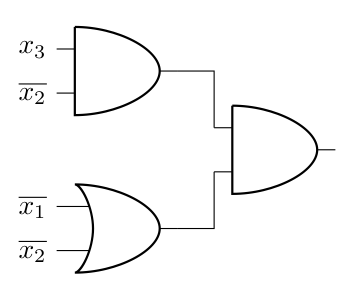
\includegraphics[scale=1]{dnf.png} \\
	\\
	\\
	KNF:\\
	\\
	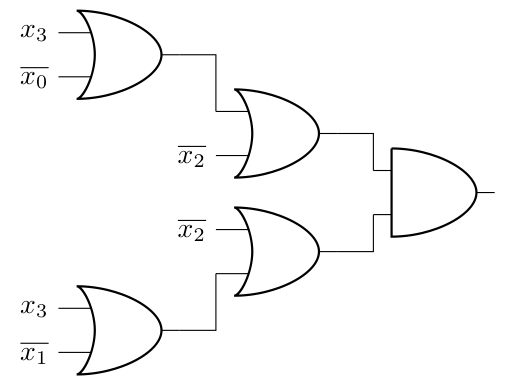
\includegraphics[scale=1]{knf.png}\\
\section{Aufgabe 8.3}
	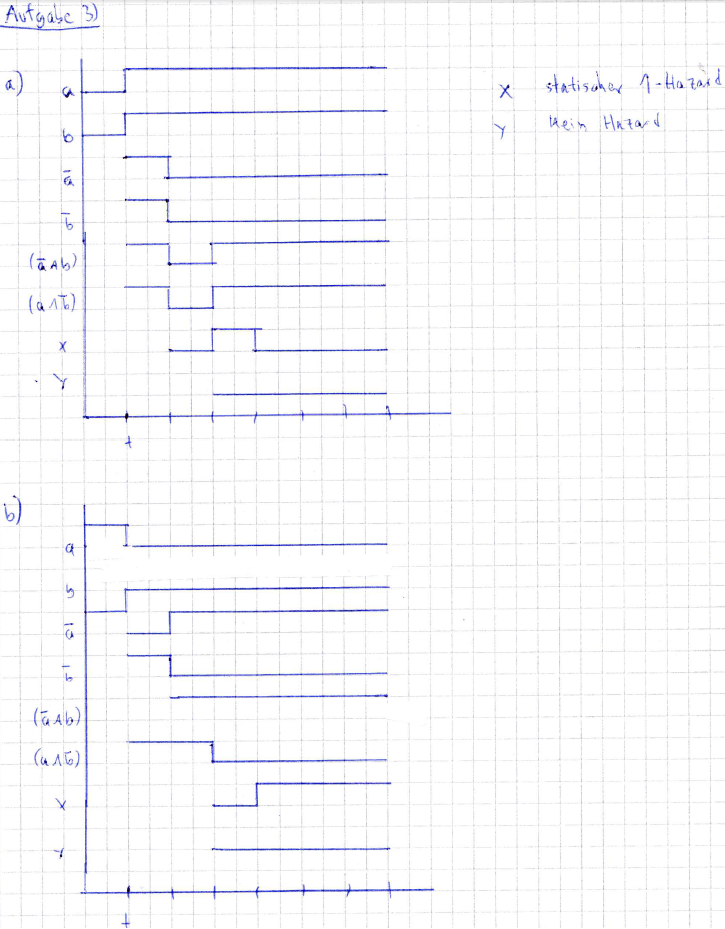
\includegraphics[scale=0.55]{8_3.png}\\
\newpage
\section{Aufgabe 8.4}
	\subsection{a)}
	Zunächst werden die generate- und propagate-Werte berechnet. Dies Kostet eine Zeiteinheit.\\
	Danach wird der CLA-Baum durchlaufen, was \textit{$log_2 (n)$} Zeiteinheiten dauert.\\
	Dann werden weitere \textit{$log_2 (n)$} Zeiteinheiten gebraucht, um die berechneten Carry-Werte zurückzureichen.\\
	Insgesamt liegt die Verzögerung also bei \textit{$2 \cdot log_2 (n) + 1$} Zeiteinheiten.
	
	\subsection{b)}
	
	Der Addierer benötigt $ f(n,m)= \dfrac{n}{m} + m - 1$\\
	Die Ableitung dieser Funktion ist: $ f'(n,m)=1-\dfrac{n}{m^2} $\\
	Daraus ergibt sich das optimale (minimale) m: $ \sqrt{n} $
	
	\subsection{c)}
	\begin{tabular}{|c|c|c|} \hline
	 \textbf{Ripple-Carry}&64bit&256bit \\ \hline
	 Verzögerung & 2,24ns  & 8,96ns \\ \hline
	 Taktrate & 446,4 MHz & 111,6 MHz \\ \hline
	\end{tabular}\\
	\\
	\\
	\\
	\begin{tabular}{|c|c|c|} \hline
	\textbf{Carry-Lookahead}&64bit&256bit \\ \hline
	Verzögerung & 455ps  & 595ps \\ \hline
	Taktrate & 2,198 GHz & 1,681 GHz \\ \hline
	\end{tabular}\\
	\\
	\\
	\\
	\begin{tabular}{|c|c|c|} \hline
	\textbf{Carry-Select}&64bit&256bit \\ \hline
	Verzögerung & 525ps  & 1,085ns \\ \hline
	Taktrate & 1,904 GHz & 921,7 MHz \\ \hline
	\end{tabular}\\
	
\end{document}